%\renewcommand{\theequation}{\theenumi}
%\begin{enumerate}[label=\arabic*.,ref=\thesubsection.\theenumi]
%\numberwithin{equation}{enumi}
%
\item The vertices of $\triangle ABC$ are $\vec{A}=\myvec{4\\6},  \vec{B}=\myvec{1\\5}$ and  $\vec{C} =  \myvec{7\\2}$.  A line is drawn to intersect sides $AB$ and $AC$ at $D$ and $E$ respectively, such that
\begin{align}
\frac{AD}{AB}=\frac{AE}{AC}= \frac{1}{4}
\end{align}
%
Find 
\begin{align}
\frac{\text{area of }\triangle ADE}{\text{area of }\triangle ABC}.
\end{align}
\solution
From the given information, 
\begin{align}
    \frac{AE}{EC} =  \frac{AD}{DB}&=\frac{1}{3}
\end{align}
and $\vec{D}$ divides AB in the ratio $1:3$ internally. $\vec{E}$ divides AE in the ratio $1:3$ internally.  Hence, 
\begin{align}
    \implies \vec{D} &=\frac{3\vec{A}+\vec{B}}{4}\\
    &=\myvec{\frac{13}{4}\\[2em]\frac{23}{4}}\\
    \vec{E} &=\frac{3\vec{A}+\vec{C}}{4}\\
    &=\myvec{\frac{19}{4}\\[2em]\frac{20}{4}}
\end{align}
\begin{align}
    \text{Area of } \triangle ABC &= \frac{1}{2}\norm{\brak{\vec{B-A}} \times \brak{\vec{C-A}}}\\
    &=\frac{1}{2}\norm{\myvec{-3\\-1}\times \myvec{3\\-4}}\\
        &=\frac{1}{2}\begin{vmatrix}
    -3&3\\
    -1&-4
    \end{vmatrix}\\
    &=\frac{1}{2}\sbrak{\brak{-3\times -4}-\brak{-1 \times 3}}\\
    &=\frac{15}{2}
\end{align}
\begin{align}
    \text{Area of } \triangle ADE &= \frac{1}{2}\norm{\brak{\vec{D-A}} \times \brak{\vec{E-A}}}\\
    &=\frac{1}{2}\norm{\myvec{\frac{-3}{4}\\[2em]\frac{-1}{4}}\times \myvec{\frac{3}{4}\\[2em]\frac{-4}{4}}}\\
    &=\frac{1}{2}\begin{vmatrix}
    \frac{-3}{4}&\frac{3}{4}\\[2em]
    \frac{-1}{4}&\frac{-4}{4}
    \end{vmatrix}\\
    &=\frac{1}{2}\sbrak{\brak{\frac{-3}{4}\times \frac{-4}{4}}-\brak{\frac{-1}{4} \times \frac{3}{4}}}\\
    &=\frac{15}{2\times16}
\end{align}
\begin{align}
    \frac{\text{area of } \triangle ADE}{\text{area of } \triangle ABC}=\frac{1}{16}
\end{align}
See Fig. \ref{aug/2/1plot}.
\begin{figure}[!h]
 \centering
 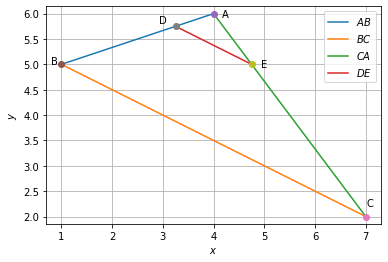
\includegraphics[width=\columnwidth]{solutions/aug/2/1/figs/figs.png}
 \caption{Plot of the triangles}
 \label{aug/2/1plot}
\end{figure}




\item In $\triangle ABC$, Show that the centroid 
\begin{align}
\vec{O} = \frac{\vec{A}+\vec{B}+\vec{C}}{3}
\end{align}
\item Check whether 
\begin{align}
\myvec{5\\-2}, \myvec{6\\4}, \myvec{7\\-2}
\end{align}
are the vertices of an isosceles triangle.
%
\\
\solution
Let,
\begin{align}
\vec{A}=\myvec{5 \\ -2}, \vec{B}=\myvec{6 \\ 4}, \vec{C}=\myvec{7 \\ -2 }\label{aug/2/5/eq:2.5.2}
\end{align}
% For the triangle to be isosceles triangle, one of\\
% \begin{align}
% 	\norm{\vec{A} - \vec{B}} =  \norm{\vec{B} - \vec{C}} \label{aug/2/5/eq:2.5.3}\\
% 	or \norm{\vec{A} - \vec{B}} =  \norm{\vec{B} - \vec{C}} \label{aug/2/5/eq:2.5.4}\\
% 	or \norm{\vec{B} - \vec{C}} =  \norm{\vec{C} - \vec{A}} \label{aug/2/5/eq:2.5.5}\\
% 	or \norm{\vec{C} - \vec{A}} =  \norm{\vec{A} - \vec{B}} \label{aug/2/5/eq:2.5.6}
% \end{align}
% Now,\\
\begin{align}
	% \vec{A-B} = \myvec{5-6 \\ (-2)-4} = \myvec{-1 \\ -6} \label{aug/2/5/eq:2.5.7}\\
 \norm{\vec{A-B}}^{2} = (-1)^{2}+(-6)^{2} = 37 \label{aug/2/5/eq:2.5.8}\\
% \vec{B-C} = \myvec{6-7 \\ 4-(-2)} = \myvec{-1 \\ 6} \label{aug/2/5/eq:2.5.9}\\
 \norm{\vec{B-C}}^{2} = (-1)^{2}+6^{2} = 37 \label{aug/2/5/eq:2.5.10}\\
% \vec{C-A} = \myvec{7-5 \\ (-2)-(-2) = \myvec{2 \\ 0}} \label{aug/2/5/eq:2.5.11}\\
% \implies \norm{\vec{C-A}}^{2} = 2^{2} = 4 \label{aug/2/5/eq:2.5.12}
\implies AB = BC
\end{align}
 
%  As 
% \begin{align}
% 	 \norm{\vec{A-B}}^{2} = \norm{\vec{B-C}}^{2} = 37 \label{aug/2/5/eq:2.5.13}
% \end{align}
% (From \eqref{aug/2/5/eq:2.5.8} and \eqref{aug/2/5/eq:2.5.10})\\
%  $\implies$ In $\Delta ABC$ sides $AB, BC$ are equal.\\
%  $\implies$ 
Hence, $\triangle ABC$ is isosceles.
 See Fig. 
%  You can also see fom the below diagram that the triangle is an isosceles triangle with sides $AB, BC$ equal.  \ref{aug/2/5/fig:2.5}

 
 \begin{figure}[h]
 	\centering
 	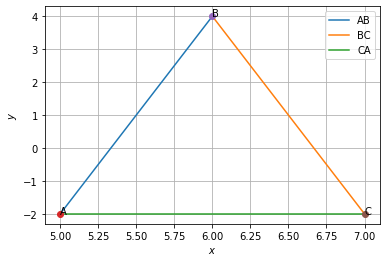
\includegraphics[width=\columnwidth]{solutions/aug/2/5/FIGURE-1.png}
 	\caption{$\Delta ABC$}
 	\label{aug/2/5/fig:2.5}
 \end{figure}

 \item Determine if the points 
\begin{align}
\myvec{1\\5}, \myvec{2\\3}, \myvec{-2\\-11}
\end{align}
%
are collinear.
\\
\solution

Let
\begin{align}
    &\vec{A} = \myvec{1\\5},\\
    &\vec{B} = \myvec{2\\3},\\
    &\vec{C} = \myvec{-2\\-11}
\end{align}
and 
\begin{align}
    \vec{M}=\myvec{\vec{B-A} & \vec{C-A}}^T
\end{align}
If $rank(\vec{M}) = 1$, the points are collinear.  The rank of a matrix is the number of nonzero rows left after doing row operations.  In this problem, 
\begin{align}
    \vec{M} = \myvec{1 & -2\\-3 & -16}\xleftrightarrow {R_2\leftarrow -\frac{R_2}{3}-R_1}\myvec{1 & -2\\0 & \frac{22}{3}}
    \\
    \implies rank(\vec{M}) = 2
    \end{align}
Therefore, the points are not collinear.  This is verified in Fig. \ref{aug/2/7/plot}.

\begin{figure}[!ht]
    \centering
    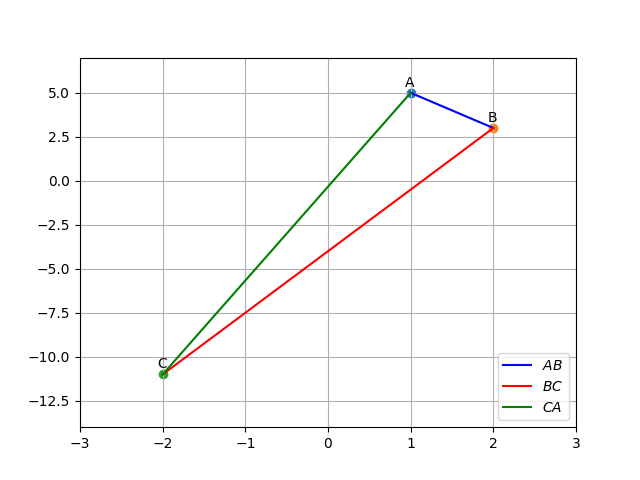
\includegraphics[width=\columnwidth]{solutions/aug/2/7/figure/figure.png}
    \caption{Plot of the points}
    \label{aug/2/7/plot}
    \end{figure}

\item By using the concept of equation of a line, prove that the three points \myvec{3\\ 0}, \myvec{– 2\\ – 2} and \myvec{8\\ 2} are collinear.
\\
\solution

\begin{table}[!ht]
\centering
\resizebox{\columnwidth}{!}{\begin{tabular}{|c|c|c|c|} 
\hline
kind of  cake & No.of cakes & Flour& Fat\\
\hline
1st & x & 200g  &  25g \\ 
\hline
2nd& y& 100g&  50g  \\ 
\hline
Total& x+y& 5 kg=5000g&1kg=1000g \\ 
\hline
\end{tabular}}
\caption{Ingredients used in making the cake is flour and fat }
\label{opt/13/tab:table1}
\end{table}
Let the  1st kind  be $x$ and the 2nd kind be $y$  such that 
\begin{align}
x \geq 0 \\
y \geq 0 
\end{align}
According to the question,
\begin{align}
2{x} + {y} \leq 50
\\
{x} + 2{y} \leq 40
\end{align}
$\therefore$ Our problem is
\begin{align}
\max_{\vec{x}} Z &= \myvec{1& 1}\vec{x}\\
s.t. \quad \myvec{2 & 1 \\ 1& 2}\vec{x} &\preceq \myvec{50\\40} 
\end{align}
Lagrangian function is given by
\begin{equation}
\begin{aligned}
&L(\vec{x},\boldsymbol{\lambda}) \\ &= \myvec{1 & 1}\vec{x}+\lcbrak{\sbrak{\myvec{2 & 1}\vec{x}-50}} \\ &+ \sbrak{\myvec{1 & 2}\vec{x}-40}\\ &+ \sbrak{\myvec{-1 & 0}\vec{x}} +\rcbrak{\sbrak{\myvec{0 & -1}\vec{x}}}\boldsymbol{\lambda}
\end{aligned}
\end{equation}
where,
\begin{align}
\boldsymbol{\lambda} &= \myvec{\lambda_1 \\ \lambda_2 \\ \lambda_3 \\ \lambda_4 \\ \lambda_5 \\ \lambda_6}
\end{align}
Now,
\begin{align}
\nabla L(\vec{x},\boldsymbol{\lambda}) &= \myvec{1+ \myvec{2 & 1 & -1 & 0 }\boldsymbol{\lambda}\\ 1+\myvec{1 & 2 & 0 & -1}\boldsymbol{\lambda} \\ \myvec{2 & 1}\vec{x}-50\\ \myvec{1& 2}\vec{x}-40 \\  \myvec{-1 & 0}\vec{x} \\ \myvec{0 & -1}\vec{x}}
\end{align}
$\therefore$ Lagrangian matrix is given by
\begin{align}
\myvec{0 & 0 & 2 & 1& -1 & 0 \\ 0 & 0 & 1 & 2  & 0 & -1 \\ 2 & 1 & 0 & 0 & 0 & 0 \\ 1 & 2 & 0 & 0 & 0 & 0  \\ -1 & 0 & 0 & 0 & 0 & 0  \\ 0 & -1 & 0 & 0 & 0 & 0 }\myvec{\vec{x} \\ \boldsymbol{\lambda} } &= \myvec{-1 \\ -1 \\ 50\\ 4 0\\ 0 \\0 }
\end{align}
Considering $\lambda_1,\lambda_2$ as only active multiplier,
\begin{align}
\myvec{0 & 0 & 2 & 1 \\ 0 & 0 & 1 & 2 \\ 2 & 1 & 0 & 0 \\ 1 & 2 & 0 & 0}\myvec{\vec{x}\\ \boldsymbol{\lambda}} &= \myvec{-1 \\ -1 \\ 5 0\\ 40}
\end{align}
resulting in,
\begin{align}
\myvec{\vec{x} \\ \boldsymbol{\lambda}} &= \myvec{0 & 0 & 2 & 1 \\ 0 & 0 & 1 & 2 \\ 2 & 1 & 0 & 0 \\ 1& 2 & 0 & 0}^{-1}\myvec{-1 \\ -1 \\ 50 \\ 40}
\\
\implies   \myvec{\vec{x} \\ \boldsymbol{\lambda}} &= \myvec{0 & 0 & \frac{2}{3} & \frac{-1}{3} \\ 0 & 0 & \frac{-1}{3} & \frac{2}{3} \\ \frac{2}{3} & \frac{-1}{3} & 0 & 0 \\ \frac{-1}{3} & \frac{2}{3} & 0 & 0}\myvec{-1 \\ -1 \\ 50 \\ 40}
\\
\implies \myvec{\vec{x} \\ \boldsymbol{\lambda}} &= \myvec{20 \\ 10 \\ -0.3 \\ -0.3 }
\end{align}
$\because \boldsymbol{\lambda}=\myvec{-0.3 \\ -0.3} \succ \vec{0} $
\\
$\therefore$ Optimal solution is given by
\begin{align}
    \vec{x} &= \myvec{20\\10} \\
    Z &= \myvec{1& 1}\vec{x} \\
    &= \myvec{1 & 1}\myvec{20 \\ 10} \\
    &= 60
\end{align}
By using cvxpy in python ,
\begin{align}
    \vec{x}=\myvec{20\\10}\\
    Z = 60
\end{align}
Hence No.of cakes \boxed{x=20} 1st kind and  .of cakes \boxed{y=10} 2nd kind should be used to maximum No. of cakes \boxed{Z=60}.  This is
verified in Fig. \ref{opt/13/fig: Graphical Solution}.	
%
\begin{figure}[!ht]
\centering
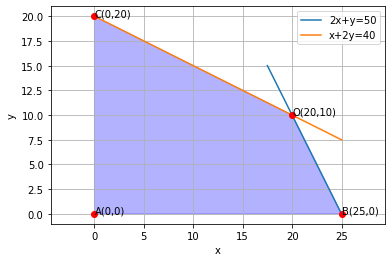
\includegraphics[width=\columnwidth]{solutions/su2021/2/13/Figure9.png}
\caption{Graphical Solution}
\label{opt/13/fig: Graphical Solution}	
\end{figure}

\item Find the value of $x$ for which the points $\myvec{x\\ – 1}$, \myvec{2\\1} and \myvec{4\\ 5} are collinear.
\\
\solution
From the given information, 
\begin{align}
    \frac{AE}{EC} =  \frac{AD}{DB}&=\frac{1}{3}
\end{align}
and $\vec{D}$ divides AB in the ratio $1:3$ internally. $\vec{E}$ divides AE in the ratio $1:3$ internally.  Hence, 
\begin{align}
    \implies \vec{D} &=\frac{3\vec{A}+\vec{B}}{4}\\
    &=\myvec{\frac{13}{4}\\[2em]\frac{23}{4}}\\
    \vec{E} &=\frac{3\vec{A}+\vec{C}}{4}\\
    &=\myvec{\frac{19}{4}\\[2em]\frac{20}{4}}
\end{align}
\begin{align}
    \text{Area of } \triangle ABC &= \frac{1}{2}\norm{\brak{\vec{B-A}} \times \brak{\vec{C-A}}}\\
    &=\frac{1}{2}\norm{\myvec{-3\\-1}\times \myvec{3\\-4}}\\
        &=\frac{1}{2}\begin{vmatrix}
    -3&3\\
    -1&-4
    \end{vmatrix}\\
    &=\frac{1}{2}\sbrak{\brak{-3\times -4}-\brak{-1 \times 3}}\\
    &=\frac{15}{2}
\end{align}
\begin{align}
    \text{Area of } \triangle ADE &= \frac{1}{2}\norm{\brak{\vec{D-A}} \times \brak{\vec{E-A}}}\\
    &=\frac{1}{2}\norm{\myvec{\frac{-3}{4}\\[2em]\frac{-1}{4}}\times \myvec{\frac{3}{4}\\[2em]\frac{-4}{4}}}\\
    &=\frac{1}{2}\begin{vmatrix}
    \frac{-3}{4}&\frac{3}{4}\\[2em]
    \frac{-1}{4}&\frac{-4}{4}
    \end{vmatrix}\\
    &=\frac{1}{2}\sbrak{\brak{\frac{-3}{4}\times \frac{-4}{4}}-\brak{\frac{-1}{4} \times \frac{3}{4}}}\\
    &=\frac{15}{2\times16}
\end{align}
\begin{align}
    \frac{\text{area of } \triangle ADE}{\text{area of } \triangle ABC}=\frac{1}{16}
\end{align}
See Fig. \ref{aug/2/1plot}.
\begin{figure}[!h]
 \centering
 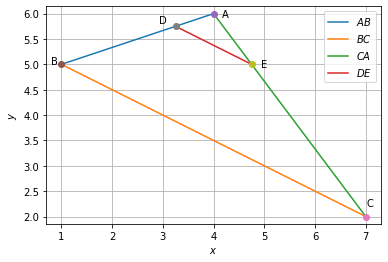
\includegraphics[width=\columnwidth]{solutions/aug/2/1/figs/figs.png}
 \caption{Plot of the triangles}
 \label{aug/2/1plot}
\end{figure}



\item  In each of the following, find the value of $k$ for which the points are collinear

\begin{enumerate}
\item \myvec{7\\-2},  \myvec{5\\1},  \myvec{3\\k} 
\item \myvec{8\\1},  \myvec{k\\-4},  \myvec{2\\-5} 
\end{enumerate}
\solution

\begin{enumerate}
\item Let $\vec{A}=\myvec{7\\-2}, \vec{B}=\myvec{5 \\ 1}, \vec{C}=\myvec{3 \\ k}$\\
The direction vectors of AB and AC are
\begin{align}
\label{aug/2/10/eq:1}
\vec{B} - \vec{A} ={}& \myvec{-2 \\ 3}\\
\label{aug/2/10/eq:2}
\vec{C} - \vec{A} ={}& \myvec{-4 \\ k+2}
\end{align}

\begin{align}
\label{aug/2/10/eq:3}
\vec{M} =\myvec{\vec{B}-\vec{A} & \vec{C}-\vec{A}}^\top
\end{align}
Substituting \eqref{aug/2/10/eq:1} and \eqref{aug/2/10/eq:2} in \eqref{aug/2/10/eq:3}, we get
\begin{align}
\label{aug/2/10/eq:4}
\vec{M}={}&\myvec{-2 & 3 \\ -4 & k+2}
\end{align}
We know that if $rank\brak{\vec{M}}=1$, the points are collinear.
Finding the rank of the matrix in the problem,
\begin{align}
\label{aug/2/10/eq:5}
\vec{M} = \myvec{-2 & 3 \\ -4 & k+2} \overset{R_{2}\rightarrow R_{2}-2R_{1}}{\longleftrightarrow} \myvec{-2 & 3 \\ 0 & k-4}
\end{align}
Since $rank\brak{\vec{M}}=1$, the number of non zero rows left after doing row operations should be equal to 1.
Since row 1 in \eqref{aug/2/10/eq:5} is non zero, elements row 2 should be equal to 0.
\begin{align}
\therefore k=4
\end{align}
\begin{figure}[!h]
\centering
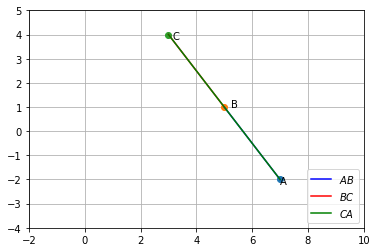
\includegraphics[width=\columnwidth]{solutions/aug/2/10/Figures/q1a.png}
\caption{Plot of the line}
\end{figure}



\item Let $\vec{A}=\myvec{8\\1}, \vec{B}=\myvec{k \\ -4}, \vec{C}=\myvec{2 \\ -5}$\\
The direction vectors of AB and AC are
\begin{align}
\label{aug/2/10/eq:7}
\vec{B} - \vec{A} ={}& \myvec{k-8\\-5}\\
\label{aug/2/10/eq:8}
\vec{C} - \vec{A} ={}& \myvec{-6 \\ -6}
\end{align}
\begin{align}
\label{aug/2/10/eq:9}
\vec{M} =\myvec{\vec{B}-\vec{A} & \vec{C}-\vec{A}}^\top
\end{align}
Substituting \eqref{aug/2/10/eq:7} and \eqref{aug/2/10/eq:8} in \eqref{aug/2/10/eq:9}, we get
\begin{align}
\label{aug/2/10/eq:10}
\vec{M}={}&\myvec{k-8 & -5 \\ -6 & -6}
\end{align}
We know that if $rank\brak{\vec{M}}=1$, the points are collinear.
Finding the rank of the matrix in the problem,
\begin{align}
\label{aug/2/10/eq:11}
\vec{M} = \myvec{k-8 & -6 \\ -5 & -6} \overset{R_{2}\rightarrow 5R_{2}-6R_{1}}{\longleftrightarrow} \myvec{k-8 & -5 \\ 18-6k & 0}
\end{align}
Since $rank\brak{\vec{M}}=1$, the number of non zero rows left after doing row operations should be equal to 1.
Since row 1 in \eqref{aug/2/10/eq:11} is non zero for any value of k , elements row 2 should be equal to 0.
\begin{align}
\therefore k=3
\end{align}

\begin{figure}[!h]
\centering
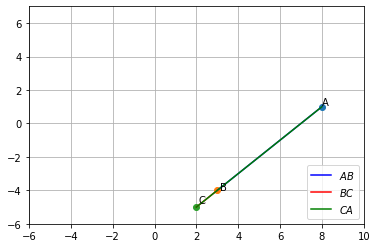
\includegraphics[width=\columnwidth]{solutions/aug/2/10/Figures/q1b.png}
\caption{Plot of the line}
\end{figure}

\end{enumerate}




\item Show that the points 
$\vec{A}=\myvec{1\\2\\7}, \vec{B}=\myvec{2\\6\\3}$ and $ \vec{C}=\myvec{3\\10\\-1}$ are collinear.
\\
\solution

\begin{table}[!ht]
\centering
\resizebox{\columnwidth}{!}{\begin{tabular}{|c|c|c|c|} 
\hline
kind of  cake & No.of cakes & Flour& Fat\\
\hline
1st & x & 200g  &  25g \\ 
\hline
2nd& y& 100g&  50g  \\ 
\hline
Total& x+y& 5 kg=5000g&1kg=1000g \\ 
\hline
\end{tabular}}
\caption{Ingredients used in making the cake is flour and fat }
\label{opt/13/tab:table1}
\end{table}
Let the  1st kind  be $x$ and the 2nd kind be $y$  such that 
\begin{align}
x \geq 0 \\
y \geq 0 
\end{align}
According to the question,
\begin{align}
2{x} + {y} \leq 50
\\
{x} + 2{y} \leq 40
\end{align}
$\therefore$ Our problem is
\begin{align}
\max_{\vec{x}} Z &= \myvec{1& 1}\vec{x}\\
s.t. \quad \myvec{2 & 1 \\ 1& 2}\vec{x} &\preceq \myvec{50\\40} 
\end{align}
Lagrangian function is given by
\begin{equation}
\begin{aligned}
&L(\vec{x},\boldsymbol{\lambda}) \\ &= \myvec{1 & 1}\vec{x}+\lcbrak{\sbrak{\myvec{2 & 1}\vec{x}-50}} \\ &+ \sbrak{\myvec{1 & 2}\vec{x}-40}\\ &+ \sbrak{\myvec{-1 & 0}\vec{x}} +\rcbrak{\sbrak{\myvec{0 & -1}\vec{x}}}\boldsymbol{\lambda}
\end{aligned}
\end{equation}
where,
\begin{align}
\boldsymbol{\lambda} &= \myvec{\lambda_1 \\ \lambda_2 \\ \lambda_3 \\ \lambda_4 \\ \lambda_5 \\ \lambda_6}
\end{align}
Now,
\begin{align}
\nabla L(\vec{x},\boldsymbol{\lambda}) &= \myvec{1+ \myvec{2 & 1 & -1 & 0 }\boldsymbol{\lambda}\\ 1+\myvec{1 & 2 & 0 & -1}\boldsymbol{\lambda} \\ \myvec{2 & 1}\vec{x}-50\\ \myvec{1& 2}\vec{x}-40 \\  \myvec{-1 & 0}\vec{x} \\ \myvec{0 & -1}\vec{x}}
\end{align}
$\therefore$ Lagrangian matrix is given by
\begin{align}
\myvec{0 & 0 & 2 & 1& -1 & 0 \\ 0 & 0 & 1 & 2  & 0 & -1 \\ 2 & 1 & 0 & 0 & 0 & 0 \\ 1 & 2 & 0 & 0 & 0 & 0  \\ -1 & 0 & 0 & 0 & 0 & 0  \\ 0 & -1 & 0 & 0 & 0 & 0 }\myvec{\vec{x} \\ \boldsymbol{\lambda} } &= \myvec{-1 \\ -1 \\ 50\\ 4 0\\ 0 \\0 }
\end{align}
Considering $\lambda_1,\lambda_2$ as only active multiplier,
\begin{align}
\myvec{0 & 0 & 2 & 1 \\ 0 & 0 & 1 & 2 \\ 2 & 1 & 0 & 0 \\ 1 & 2 & 0 & 0}\myvec{\vec{x}\\ \boldsymbol{\lambda}} &= \myvec{-1 \\ -1 \\ 5 0\\ 40}
\end{align}
resulting in,
\begin{align}
\myvec{\vec{x} \\ \boldsymbol{\lambda}} &= \myvec{0 & 0 & 2 & 1 \\ 0 & 0 & 1 & 2 \\ 2 & 1 & 0 & 0 \\ 1& 2 & 0 & 0}^{-1}\myvec{-1 \\ -1 \\ 50 \\ 40}
\\
\implies   \myvec{\vec{x} \\ \boldsymbol{\lambda}} &= \myvec{0 & 0 & \frac{2}{3} & \frac{-1}{3} \\ 0 & 0 & \frac{-1}{3} & \frac{2}{3} \\ \frac{2}{3} & \frac{-1}{3} & 0 & 0 \\ \frac{-1}{3} & \frac{2}{3} & 0 & 0}\myvec{-1 \\ -1 \\ 50 \\ 40}
\\
\implies \myvec{\vec{x} \\ \boldsymbol{\lambda}} &= \myvec{20 \\ 10 \\ -0.3 \\ -0.3 }
\end{align}
$\because \boldsymbol{\lambda}=\myvec{-0.3 \\ -0.3} \succ \vec{0} $
\\
$\therefore$ Optimal solution is given by
\begin{align}
    \vec{x} &= \myvec{20\\10} \\
    Z &= \myvec{1& 1}\vec{x} \\
    &= \myvec{1 & 1}\myvec{20 \\ 10} \\
    &= 60
\end{align}
By using cvxpy in python ,
\begin{align}
    \vec{x}=\myvec{20\\10}\\
    Z = 60
\end{align}
Hence No.of cakes \boxed{x=20} 1st kind and  .of cakes \boxed{y=10} 2nd kind should be used to maximum No. of cakes \boxed{Z=60}.  This is
verified in Fig. \ref{opt/13/fig: Graphical Solution}.	
%
\begin{figure}[!ht]
\centering
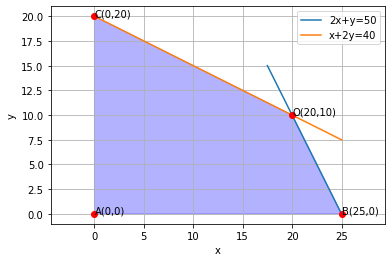
\includegraphics[width=\columnwidth]{solutions/su2021/2/13/Figure9.png}
\caption{Graphical Solution}
\label{opt/13/fig: Graphical Solution}	
\end{figure}

\item Show that the points 
$\vec{A}=\myvec{1\\-2\\-8}, \vec{B}=\myvec{5\\0\\-2}$ and $ \vec{C}=\myvec{11\\3\\7}$ are collinear, and find the ratio in which $\vec{B}$ divides $AC$.
\\
\solution
From the given information, 
\begin{align}
    \frac{AE}{EC} =  \frac{AD}{DB}&=\frac{1}{3}
\end{align}
and $\vec{D}$ divides AB in the ratio $1:3$ internally. $\vec{E}$ divides AE in the ratio $1:3$ internally.  Hence, 
\begin{align}
    \implies \vec{D} &=\frac{3\vec{A}+\vec{B}}{4}\\
    &=\myvec{\frac{13}{4}\\[2em]\frac{23}{4}}\\
    \vec{E} &=\frac{3\vec{A}+\vec{C}}{4}\\
    &=\myvec{\frac{19}{4}\\[2em]\frac{20}{4}}
\end{align}
\begin{align}
    \text{Area of } \triangle ABC &= \frac{1}{2}\norm{\brak{\vec{B-A}} \times \brak{\vec{C-A}}}\\
    &=\frac{1}{2}\norm{\myvec{-3\\-1}\times \myvec{3\\-4}}\\
        &=\frac{1}{2}\begin{vmatrix}
    -3&3\\
    -1&-4
    \end{vmatrix}\\
    &=\frac{1}{2}\sbrak{\brak{-3\times -4}-\brak{-1 \times 3}}\\
    &=\frac{15}{2}
\end{align}
\begin{align}
    \text{Area of } \triangle ADE &= \frac{1}{2}\norm{\brak{\vec{D-A}} \times \brak{\vec{E-A}}}\\
    &=\frac{1}{2}\norm{\myvec{\frac{-3}{4}\\[2em]\frac{-1}{4}}\times \myvec{\frac{3}{4}\\[2em]\frac{-4}{4}}}\\
    &=\frac{1}{2}\begin{vmatrix}
    \frac{-3}{4}&\frac{3}{4}\\[2em]
    \frac{-1}{4}&\frac{-4}{4}
    \end{vmatrix}\\
    &=\frac{1}{2}\sbrak{\brak{\frac{-3}{4}\times \frac{-4}{4}}-\brak{\frac{-1}{4} \times \frac{3}{4}}}\\
    &=\frac{15}{2\times16}
\end{align}
\begin{align}
    \frac{\text{area of } \triangle ADE}{\text{area of } \triangle ABC}=\frac{1}{16}
\end{align}
See Fig. \ref{aug/2/1plot}.
\begin{figure}[!h]
 \centering
 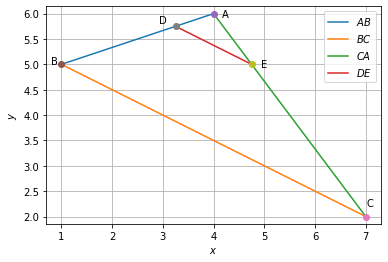
\includegraphics[width=\columnwidth]{solutions/aug/2/1/figs/figs.png}
 \caption{Plot of the triangles}
 \label{aug/2/1plot}
\end{figure}



\item Show that 
$
\vec{A}=\myvec{2\\3\\4}, 
\vec{B}=\myvec{-1\\-2\\1} \text{ and } 
\vec{C}=\myvec{5\\8\\7}$  
are collinear.
\\
\solution
%
If solution exists for the given
system of equations then they
said to be consistent, otherwise they are
inconsistent.
The above equations can be expressed as the matrix equation
\begin{align}
\myvec{1 & 2\\2 & 3} \vec{x} = \myvec{2\\3}
\end{align}
%
The augmented matrix for the above equation and row reducing as follows
\begin{align}
\myvec{1 & 2 & 2 \\ 2 & 3 & 3}  \xleftrightarrow[]{R_2\rightarrow R_2-2R_1} \myvec{1 & 2 & 2 \\ 0 & -1 & -1}\\
\xleftrightarrow[]{R_1\rightarrow R_1+2R_2}
\myvec{1 & 0 & 0\\0 & -1 & -1}\label{aug/2/70/a}\\
\implies\text{Rank}\myvec{1&2\\2&3}=\text{Rank}\myvec{1&2&2\\2&3&3}=2
\end{align}
Here, $Rank(A)=Rank(A|B)$. Therefore, the system is consistent. Also, there exist a unique solution as $Rank(A)=n$ (number of unknown).\\ 
From equation \eqref{aug/2/70/a}, we get:
\begin{align}
    \vec{x}=\myvec{0\\1}
\end{align}
Plotting the lines and the intersection point in Fig.\ref{aug/2/70/b}
\begin{figure}[htp]
\centering
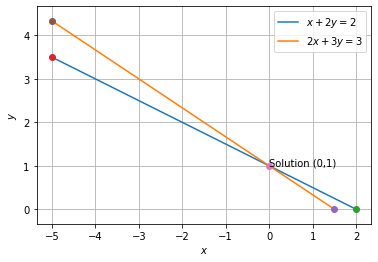
\includegraphics[width=\columnwidth]{solutions/aug/2/70/a_2.png}
\caption{Lines and their intersection denoting the solution}
\label{aug/2/70/b}
\end{figure}
%
$\therefore$ The given system of equation is consistent with unique solution of,
$$\myvec{x\\y}=\myvec{0\\1}$$


\item A bullet fired at an angle of 30$\degree$ with the horizontal hits the ground 3.0 km away. By adjusting its angle of projection, can one hope to hit a target 5.0 km away ? Assume the muzzle speed to be fixed, and neglect air resistance.
\item  A fighter plane flying horizontally at an altitude of 1.5 km with speed 720 km/h passes directly overhead an anti-aircraft gun. At what angle from the vertical should the gun be fired for the shell with muzzle speed 600 $m s^{-1}$ to hit the plane ? 
At what minimum  altitude should the pilot fly the plane to avoid being hit ? (Take g = 10$ m s^{-2}$
).
\item Give the magnitude and direction of the net force acting on a stone of mass 0.1 kg, 
\begin{enumerate}
\item  just after it is dropped from the window of a stationary train, 
\item  just after it is dropped from the window of a train running at a constant velocity of 36 km/h,
\item  just after it is dropped from the window of a train accelerating with 1$ m s^{-2} $
\item  lying on the floor of a train which is accelerating with 1 $m s^{-2}$, the stone being at rest relative to the train.
\end{enumerate}
Neglect air resistance throughout. 

\item Consider the collision depicted in Fig. \ref{fig:6.10} to be between two billiard balls with equal masses $m_1= m_2$.  The first ball is called the cue while the second ball is called the target. The billiard player wants to 'sink' the target ball in a corner pocket, which is at an angle $\theta_2=37\degree$.  Assume that the collosion
is elastic and that friction and rotational motion are not important. Obtain $\theta_1$.
\begin{figure}[!ht]
\centering
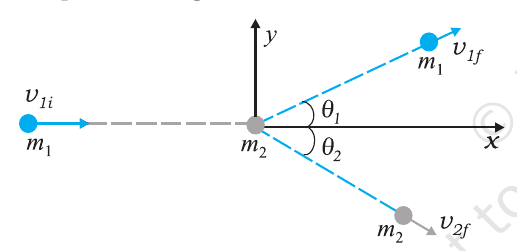
\includegraphics[width=\columnwidth]{./line/figs/11-1/6/6.10.eps}
\caption{}
\label{fig:6.10}
\end{figure}
%
\item Find the ratio in which the line segment joining the points \myvec{4\\8\\10} and \myvec{6\\10\\-8} is divided by the YZ-plane.
%
\\
\solution

\begin{table}[!ht]
\centering
\resizebox{\columnwidth}{!}{\begin{tabular}{|c|c|c|c|} 
\hline
kind of  cake & No.of cakes & Flour& Fat\\
\hline
1st & x & 200g  &  25g \\ 
\hline
2nd& y& 100g&  50g  \\ 
\hline
Total& x+y& 5 kg=5000g&1kg=1000g \\ 
\hline
\end{tabular}}
\caption{Ingredients used in making the cake is flour and fat }
\label{opt/13/tab:table1}
\end{table}
Let the  1st kind  be $x$ and the 2nd kind be $y$  such that 
\begin{align}
x \geq 0 \\
y \geq 0 
\end{align}
According to the question,
\begin{align}
2{x} + {y} \leq 50
\\
{x} + 2{y} \leq 40
\end{align}
$\therefore$ Our problem is
\begin{align}
\max_{\vec{x}} Z &= \myvec{1& 1}\vec{x}\\
s.t. \quad \myvec{2 & 1 \\ 1& 2}\vec{x} &\preceq \myvec{50\\40} 
\end{align}
Lagrangian function is given by
\begin{equation}
\begin{aligned}
&L(\vec{x},\boldsymbol{\lambda}) \\ &= \myvec{1 & 1}\vec{x}+\lcbrak{\sbrak{\myvec{2 & 1}\vec{x}-50}} \\ &+ \sbrak{\myvec{1 & 2}\vec{x}-40}\\ &+ \sbrak{\myvec{-1 & 0}\vec{x}} +\rcbrak{\sbrak{\myvec{0 & -1}\vec{x}}}\boldsymbol{\lambda}
\end{aligned}
\end{equation}
where,
\begin{align}
\boldsymbol{\lambda} &= \myvec{\lambda_1 \\ \lambda_2 \\ \lambda_3 \\ \lambda_4 \\ \lambda_5 \\ \lambda_6}
\end{align}
Now,
\begin{align}
\nabla L(\vec{x},\boldsymbol{\lambda}) &= \myvec{1+ \myvec{2 & 1 & -1 & 0 }\boldsymbol{\lambda}\\ 1+\myvec{1 & 2 & 0 & -1}\boldsymbol{\lambda} \\ \myvec{2 & 1}\vec{x}-50\\ \myvec{1& 2}\vec{x}-40 \\  \myvec{-1 & 0}\vec{x} \\ \myvec{0 & -1}\vec{x}}
\end{align}
$\therefore$ Lagrangian matrix is given by
\begin{align}
\myvec{0 & 0 & 2 & 1& -1 & 0 \\ 0 & 0 & 1 & 2  & 0 & -1 \\ 2 & 1 & 0 & 0 & 0 & 0 \\ 1 & 2 & 0 & 0 & 0 & 0  \\ -1 & 0 & 0 & 0 & 0 & 0  \\ 0 & -1 & 0 & 0 & 0 & 0 }\myvec{\vec{x} \\ \boldsymbol{\lambda} } &= \myvec{-1 \\ -1 \\ 50\\ 4 0\\ 0 \\0 }
\end{align}
Considering $\lambda_1,\lambda_2$ as only active multiplier,
\begin{align}
\myvec{0 & 0 & 2 & 1 \\ 0 & 0 & 1 & 2 \\ 2 & 1 & 0 & 0 \\ 1 & 2 & 0 & 0}\myvec{\vec{x}\\ \boldsymbol{\lambda}} &= \myvec{-1 \\ -1 \\ 5 0\\ 40}
\end{align}
resulting in,
\begin{align}
\myvec{\vec{x} \\ \boldsymbol{\lambda}} &= \myvec{0 & 0 & 2 & 1 \\ 0 & 0 & 1 & 2 \\ 2 & 1 & 0 & 0 \\ 1& 2 & 0 & 0}^{-1}\myvec{-1 \\ -1 \\ 50 \\ 40}
\\
\implies   \myvec{\vec{x} \\ \boldsymbol{\lambda}} &= \myvec{0 & 0 & \frac{2}{3} & \frac{-1}{3} \\ 0 & 0 & \frac{-1}{3} & \frac{2}{3} \\ \frac{2}{3} & \frac{-1}{3} & 0 & 0 \\ \frac{-1}{3} & \frac{2}{3} & 0 & 0}\myvec{-1 \\ -1 \\ 50 \\ 40}
\\
\implies \myvec{\vec{x} \\ \boldsymbol{\lambda}} &= \myvec{20 \\ 10 \\ -0.3 \\ -0.3 }
\end{align}
$\because \boldsymbol{\lambda}=\myvec{-0.3 \\ -0.3} \succ \vec{0} $
\\
$\therefore$ Optimal solution is given by
\begin{align}
    \vec{x} &= \myvec{20\\10} \\
    Z &= \myvec{1& 1}\vec{x} \\
    &= \myvec{1 & 1}\myvec{20 \\ 10} \\
    &= 60
\end{align}
By using cvxpy in python ,
\begin{align}
    \vec{x}=\myvec{20\\10}\\
    Z = 60
\end{align}
Hence No.of cakes \boxed{x=20} 1st kind and  .of cakes \boxed{y=10} 2nd kind should be used to maximum No. of cakes \boxed{Z=60}.  This is
verified in Fig. \ref{opt/13/fig: Graphical Solution}.	
%
\begin{figure}[!ht]
\centering
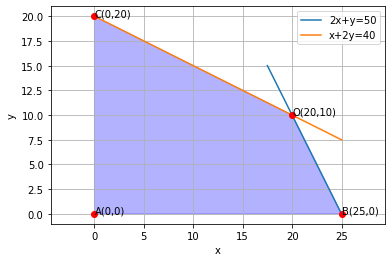
\includegraphics[width=\columnwidth]{solutions/su2021/2/13/Figure9.png}
\caption{Graphical Solution}
\label{opt/13/fig: Graphical Solution}	
\end{figure}

%\\
%\solution Use \eqref{eq:line_section_form}.  The YZ-plane has points \myvec{0\\y\\z}.
%

%
%\\
%\solution Use the approach in Problem \ref{prob:line_perp_bisect}.
\item If 
\begin{align}
\vec{P} = 3\vec{a}-2\vec{b}
\\
\vec{Q} = \vec{a}+\vec{b}
\end{align}
%
find $\vec{R}$, which divides $PQ$ in the ratio $2:1$
\begin{enumerate}
\item internally,
\item externally.
\end{enumerate}
%
%
\item Find a unit vector in the direction of $\vec{A}+\vec{B}$, where 
%
\begin{align}
\vec{A} = \myvec{2\\2\\-5}, \vec{B} = \myvec{2\\1\\3}.
\end{align}
%
\solution
Let $\vec{C}$ be the vector $\vec{A} + \vec{B}$
\begin{align}
    \vec{C} &= \vec{A} + \vec{B} \\
    \therefore \vec{C} &= \myvec{4\\3\\-2}\\
\text{Now,}\notag\\
    \norm{\vec{C}} &= \sqrt{(4)^2 + (3)^2 + (-2)^2}\\
    \therefore \norm{\vec{C}} &= \sqrt{29}
\end{align}
\\Let $\vec{H}$ be the unit vector in the direction of $\vec{C}$.
\begin{align}
    \vec{H} &= \dfrac{\vec{C}}{\norm{\vec{C}}}\\
    \therefore \vec{H} &= \dfrac{1}{\sqrt{29}} \myvec{4\\3\\-2}
\end{align}
Hence, $\vec{H}$ is the required unit vector.
%\end{enumerate}
%

